% https://topanswers.xyz/tex?q=770#a897
\documentclass[8pt]{beamer}
\usefonttheme{serif}
%\usepackage{multicol}
%\usepackage{minted}
\usepackage{tikz}
\usecolortheme{dove}
%\columnseprule=0.01em

\usetikzlibrary{tikzmark,calc}

\begin{document}
\begin{frame}{First}

\tikzmark{start}
\begin{columns}[onlytextwidth,c]
\begin{column}{.45\textwidth}
This is some text. This is some text. This is some text. This is some text. This is some text. This is some text. This is some text. This is some text. This is some text. This is some text. This is some text. This is some text. This is some text. This is some text. This is some text.
\end{column}
\begin{column}{8mm}
\begin{tikzpicture}[remember picture, overlay, inner sep=0pt,outer sep=0pt]
	\draw<1> let \p{A}=(pic cs:start), \p{B}=(pic cs:stop) in
    (4mm,\y{A}) -- (4mm,\y{B});
	\draw<2-> let \p{A}=(pic cs:start), \p{B}=(pic cs:stop) in
    (4mm,\y{A}) -- (4mm,\y{B}) node[midway,circle,draw,fill=white,text width=8mm,align=center] (b) {text};
	\end{tikzpicture}
\end{column}
\begin{column}{.45\textwidth}
\uncover<3->{This is some text. This is some text. This is some text. This is some text. This is some text.}
\end{column}
\end{columns}
\tikzmark{stop}

\end{frame}
\end{document}